\documentclass[]{scrartcl}
\usepackage{lmodern}
\usepackage{amssymb,amsmath}
\usepackage{ifxetex,ifluatex}
\usepackage{fixltx2e} % provides \textsubscript
\ifnum 0\ifxetex 1\fi\ifluatex 1\fi=0 % if pdftex
  \usepackage[T1]{fontenc}
  \usepackage[utf8]{inputenc}
\else % if luatex or xelatex
  \ifxetex
    \usepackage{mathspec}
  \else
    \usepackage{fontspec}
  \fi
  \defaultfontfeatures{Ligatures=TeX,Scale=MatchLowercase}
\fi
% use upquote if available, for straight quotes in verbatim environments
\IfFileExists{upquote.sty}{\usepackage{upquote}}{}
% use microtype if available
\IfFileExists{microtype.sty}{%
\usepackage{microtype}
\UseMicrotypeSet[protrusion]{basicmath} % disable protrusion for tt fonts
}{}
\usepackage{hyperref}
\hypersetup{unicode=true,
            pdftitle={Angabe},
            pdfauthor={Team\ldots{}},
            pdfborder={0 0 0},
            breaklinks=true}
\urlstyle{same}  % don't use monospace font for urls
\IfFileExists{parskip.sty}{%
\usepackage{parskip}
}{% else
\setlength{\parindent}{0pt}
\setlength{\parskip}{6pt plus 2pt minus 1pt}
}
\setlength{\emergencystretch}{3em}  % prevent overfull lines
\providecommand{\tightlist}{%
  \setlength{\itemsep}{0pt}\setlength{\parskip}{0pt}}
\setcounter{secnumdepth}{5}
% Redefines (sub)paragraphs to behave more like sections
\ifx\paragraph\undefined\else
\let\oldparagraph\paragraph
\renewcommand{\paragraph}[1]{\oldparagraph{#1}\mbox{}}
\fi
\ifx\subparagraph\undefined\else
\let\oldsubparagraph\subparagraph
\renewcommand{\subparagraph}[1]{\oldsubparagraph{#1}\mbox{}}
\fi

\usepackage{graphicx}
\usepackage{array}
\usepackage{ragged2e}
\usepackage[section]{placeins}
\makeatletter
\AtBeginDocument{%
  \expandafter\renewcommand\expandafter\subsection\expandafter{%
    \expandafter\@fb@secFB\subsection
  }%
}
\makeatother

\title{Modell eines Insel-Callshops}
\providecommand{\subtitle}[1]{}
\subtitle{2. Projekt zu Modellierung und Simulation}
\author{Daniel Graf, Dimitrie Diez, Arne Schöntag, Peter Müller}
\date{}

\begin{document}

\maketitle

\tableofcontents
\section{Einführung}
Simulationen haben in der moderne einen sehr hohen Stellenwert erlangt, da durch sie zahlreiche, oftmals sehr genaue, Zukunftsprognosen erstellt werden können. Als Grundlage für die Simulationen dienen in der Regel Modelle, welche einen Ausschnitt der Wirklichkeit abbilden. Das Thema dieser Studienarbeit ist die Simulation eines Callshops, bzw. des Telefons in einem Callshop, in einem Inseldorf. Dieser wird für günstige Telefonate ins Ausland verwendet. 

\section{Beschreibung des Modells}
Für die Simulation des Insel-Callshops wird ein Warteschlagenmodell mit Clients und zunächst nur einem Server verwendet. Jede Person die den CallShop betritt wird durch einen neuen Client repräsentiert. Das Telefon des Shops ist durch den Server dargestellt. Möchte eine Person das Telefon zu einem Zeitpunkt benützen, zu dem bereits eine andere Person telefoniert, muss sie sich hinten anstellen und warten, bis die Person ihr Telefonat beendet hat. Im Modell wird dieses durch eine Warteschlage (Queue) realisiert, in die sich ankommende Clients einordnen und sobald der Server nichtmehr belegt ist nach dem FIFO (first in first out) Prinzip bedient werden. 

Im Modell werden sowohl die Ankunftszeiten der Clients, als auch die Dauer der Telefonate durch eine negative Exponentialverteilung beschrieben, da diese sehr nah an den real beoachteten Verhalten liegt. Der mathematische Hintergrund liegt in der Eigenschaft der Exponentialfunktion zugrunde. Die Exponentialverteilung ist die einzige kontinuierliche Verteilung, welche zugleich die Markoveigenschaft, die sogenannte Gedächtnislosigkeit, erfüllt. Diese besagt, dass die seit dem letzten Ereignis vergangene Zeit (in diesem Beispiel Anrufer) keinen Einfluss auf die Verteilung der Zeit bis zum nächsten Ereignis (bis zum nächsten Anruf) hat. 
Quelle: http://www.mathepedia.de/Exponentialverteilung.aspx

Darüber hinaus wird ein zweites Modell betrachtet, in welchem die Bewohner des Inseldorfes (Einheimische) bevorzugt werden. Im weiteren Verlauf der Studienarbeit werden diese mit VIP bezeichnet. 

In einem dritten Modell befindet sich ein weiteres Telefon im Callshop. Von den nun zwei Telefonen (zwei Server), behandelt eines alle ankommenden Personen (Clients) gleichberechtigt. Das zweite Telefon bevorzugt die VIPs und behandelt andere Personen nur, wenn kein VIP wartet.

\section{Anforderungen/Requirements}

\section{Softwaredesign}

\section{Softwaretest}

\section{Auswertung der Ergebnisse}
Im Zuge dieses Kapitels werden alle Ergebnisse der Simulation und die daraus errechneten Werte erläutert. Zusätzlich werden relevante Größen durch Plots veranschaulicht.

\subsection{Modell \glqq Ein Telefon\grqq} 
Für den in Kapitel \ref{sec:Requirements} REFERENZAUFANFORDERUNG aufgelisteten ersten Betriebsmodus (ein Server, welcher alle Clients bedient) werden im folgenden die Auswertungen aufgeführt. Exemplarisch werden vier verschiedene durchschnittliche Ankunftszeiten für die Clients verwendet. Zunächst wird eine durchschnittliche Ankunftszeit von 1500 angenommen, was bei einer durchschnittlichen Telefonierdauer (Dauer der Serverbelegung) einer sehr geringen Serverauslastung entspricht. Anschließend werden mit den durchschnittlichen Ankunftszeiten von 1000, 500 und 100 die Auswirkungen von höherer Serverauslastung auf das Ergebnis der Simulation erläutert. \\

Für jede durchschnittliche Ankunftszeit werden zunächst die zu erwartenden Werte, basierend auf den Formeln für M/M/1 Warteschlangenmodelle ermittelt. Die einzelnen Formeln sind im folgenden Kapitel aufgeführt. Betrachtet werden hierbei, wie in den \ref{sec:Requirements} erläutert die durchschnittliche Anzahl von Kunden im System, durchschnittliche Warteschlangenlänge, durchschnittliche Verweildauer im System und die durchschnittliche Verweildauer in der Warteschlange. Die berechneten Größen werden als Erwartungswerte betrachtet gegen die die durch die Simulation ermittelten Werte geprüft werden. 

Sowohl die Maßnahmen für die Verifikation der implementierten Simulation, als auch für die Validierung der errechneten Durschnittswerte, werden in den Kapitel (REFERENZ AUF DIE ZWEI KAPITEL) näher beschrieben. In den folgenden Abbildungen wird die durchschnittliche Zwischenankunftszeit mit \glqq MeanAr\grqq abgekürzt.

%\subsubsection{Durchschnittliche Ankunftszeit der Clients: 1500}
%\paragraph{Verwendung der Mathematica Simulation}
%- Bild der Simulation 
%- Plot Little-Law
%- MeanSystemSize, MeanSystemTime, MeanQueueSize,MeanQueueTime aufführen
%
%\paragraph{Verwendung der implementierten Java-Simulation, Berechnung in Mathematica}
%\begin{figure}[htpb]
%	\centering
%	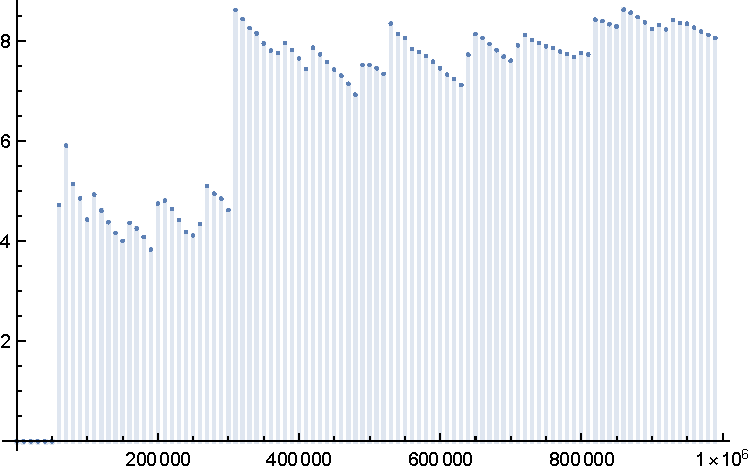
\includegraphics[width=0.8\textwidth]{abbildungen/auswertung1500/meanQueueTimePlot.pdf}
%	\caption{Mittlere Warteschlangenlänge, MeanAr = 1500}
%	\label{fig:meanQueueTime1500}
%\end{figure}
%
%\begin{figure}[htpb]
%	\centering
%	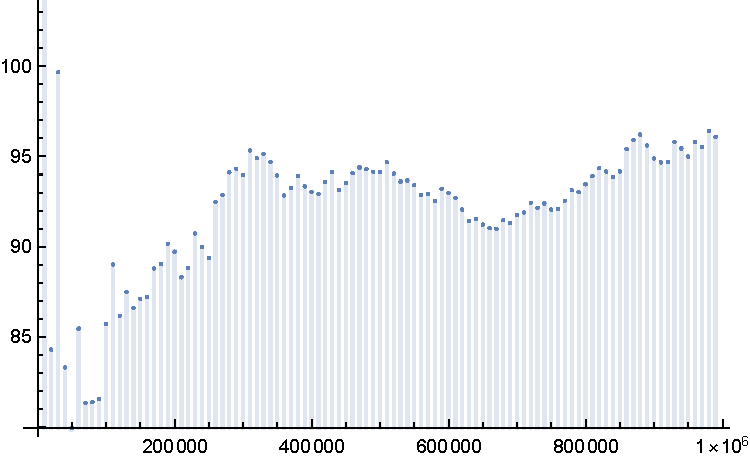
\includegraphics[width=0.8\textwidth]{abbildungen/auswertung1500/meanCallingTimePlot.pdf}
%	\caption{Mittlere Telefonierdauer, MeanAr = 1500}
%	\label{fig:meanCallingTime1500}
%\end{figure}
%
%\begin{figure}[htpb]
%	\centering
%	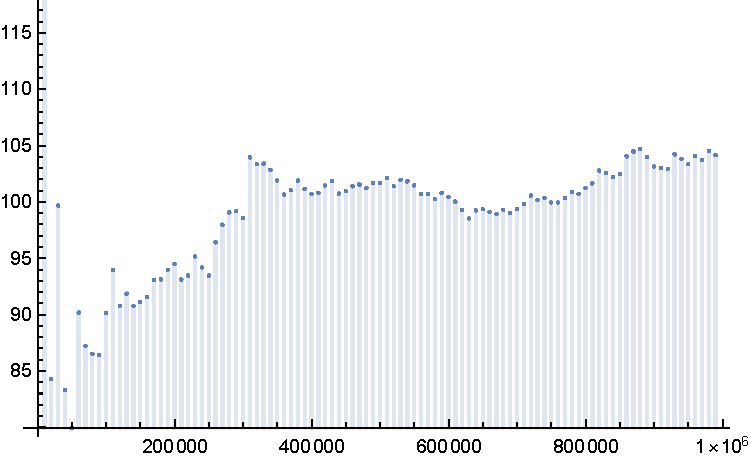
\includegraphics[width=0.8\textwidth]{abbildungen/auswertung1500/meanSystemTimePlot.pdf}
%	\caption{Mittlere Zeit im System (Wartezeit + Telefonierdauer), MeanAr = 1500}
%	\label{fig:meanSystemTime1500}
%\end{figure}
%\paragraph{Simulation und Berechnung in Java}

\subsubsection{Formeln für M/M/1 Warteschlangenmodelle}
\label{Formeln}
Die im folgenden aufgeführten Formeln gelten für M/M/1 Warteschlangenmodelle. Mit $Ls$ wird die durchschnittliche Anzahl von Kunden im System bezeichnet. $Lq$ gibt die durchschnittliche Länge der Warteschlange an. $Ws$ definiert die durchschnittliche Verweildauer der einzelnen Kunden im System und $Wq$ die durchschnittliche Verweildauer in der Warteschlange. 

\begin{equation}
Ls=\frac{\lambda}{\mu - \lambda}
\end{equation}
\begin{equation}
Lq=\frac{\rho\lambda}{\mu - \lambda}
\end{equation}
\begin{equation}
Ws=\frac{1}{\mu - \lambda}
\end{equation}
\begin{equation}
Wq=\frac{\rho}{\mu - \lambda}
\end{equation}
In den einzelnen Gleichungen beschreibt $\lambda$, $\mu$ und $\rho$ wie folgt definiert: $\lambda$ beschreibt die durchschnittliche Ankunftszeit der Kunden pro Zeiteinheit. $\mu$ definiert die durchschnittliche Telefonierdauer der Kunden pro Zeiteinheit. Und $\rho$ beschreibt die durchschnittliche Auslastung des Telefons. Quelle: $http://www.business.uzh.ch/dam/jcr:00000000-0451-792f-ffff-fffffe13aac9/ServiceManagement_Warteschlangenmodelle.pdf$

\begin{equation}
\rho=\frac{\lambda}{\mu}
\end{equation}
\subsubsection{Validierung der einzelnen Auswertung auf Basis des Little Theorems}
Laut dem Theorem von Little muss die durchschnittliche Anzahl von Kunden in einem Warteschlangensystem gleich dem Produkt aus der durchschnittlichen Ankunftsrate ($\Lambda$) und der durchschnittlichen Verweildauer ($Ws$) im System sein, wenn das System sich in einem eingeschwungenen Zustand befindet.
\begin{equation}
Ls=\lambda*Ws
\end{equation}
Stellt man die Formel um, muss im eingeschwungenen Zustand gelten:
\begin{equation}
\label{eq:little}
\lambda*Ws - Ls=0
\end{equation}
Anhand dieser Gleichung werden im weiteren Verlauf der Studienarbeit die einzelnen Auswertungen validiert.

\subsubsection{Durchschnittliche Zwischenankunftszeit der Clients: 1000}
\paragraph{Theoretische Erwartungswerte laut M/M/1 Warteschlangenmodell}
Bei einer durchschnittlichen Zwischenankunftszeit von 1000 ($\lambda=\frac{1}{1000}$, $\mu=\frac{1}{100}$)ergeben sich, basierend auf den in Abschnitt \label{Formeln} aufgeführten Formeln, folgende Erwartungswerte:
\begin{equation}
Ls=0,111111
\end{equation}
\begin{equation}
Lq=0,0111111
\end{equation}
\begin{equation}
Ws=111,111
\end{equation}
\begin{equation}
Wq=11,1111
\end{equation}
Die einzelnen Erwartungswerte sind in den nachfolgenden Plots durch eine gelbe Linie hervorgehoben.
\paragraph{Verwendung der implementierten Java-Simulation, Berechnung in Java}

\begin{figure}[htpb]
	\centering
	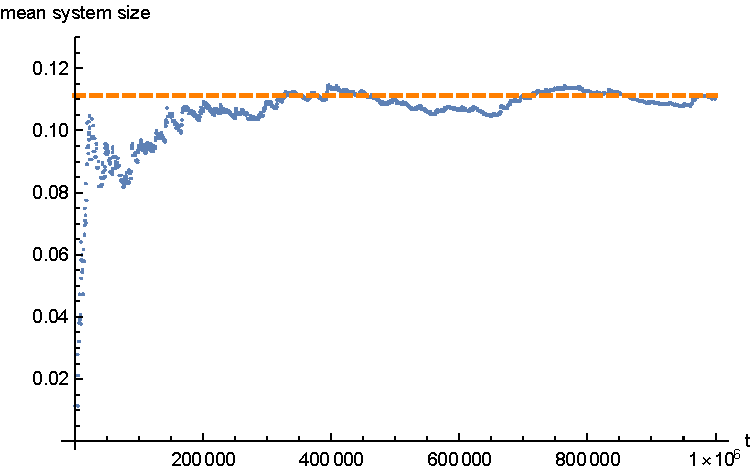
\includegraphics[width=0.8\textwidth]{abbildungen/1_Phone/Arrival_1000_Serve_100_dur_1000000_Skip_0/MeanSystemSize.pdf}
	\caption{Durchschnittliche Anzahl an Kunden im System, MeanAr = 1000}
	\label{fig:meanSystemSize1000}
\end{figure}

Abbildung \ref{fig:meanSystemSize1000} zeigt die durchschnittliche Anzahl an Kunden im System an. Ab einer Simulationszeit von ca $200000$ liegt diese konstant bei $0.111111$, was mit dem Erwartungswert übereinstimmt und somit ein Indiz für die Richtigkeit der Simulation darstellt. Durch die Vergleichsweise kurze Telefonierzeit und lange Zwischenankunftszeit befinden sich über den Zeitverlauf nur wenige Kunden im System. 

\begin{figure}[htpb]
	\centering
	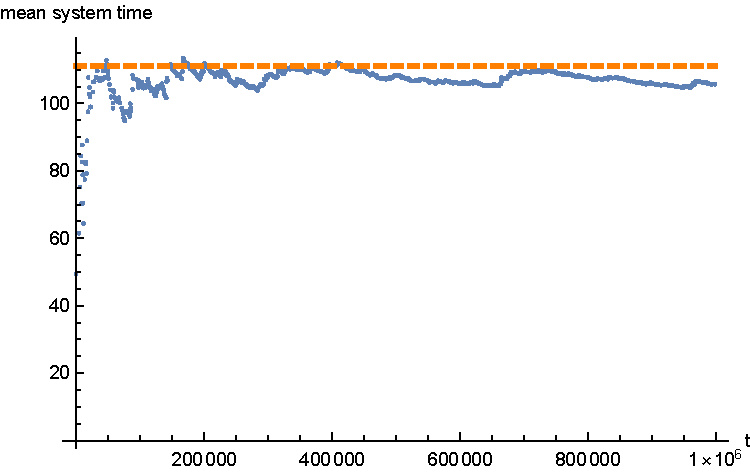
\includegraphics[width=0.8\textwidth]{abbildungen/1_Phone/Arrival_1000_Serve_100_dur_1000000_Skip_0/MeanSystemTime.pdf}
	\caption{Durchschnittliche Verweildauer der Kunden im System, MeanAr = 1000}
	\label{fig:meanSystemTime1000}
\end{figure}

Betrachtet man Abbildung \ref{fig:meanSystemTime1000}, wird deutlich, dass die durchschnittliche Verweilsdauer im System bis zu einer Simulationszeit von $300000$ noch stark variiert. Anschließend ändert sie sich nur noch geringfügig, bleibt jedoch unter dem erwarteten Wert von $111.111$. Der Grund hierfür könnte entweder eine Ungenauigkeit aufgrund von Runden bei der Division oder ein Fehler in der Berechnung sein.

\begin{figure}[htpb]
	\centering
	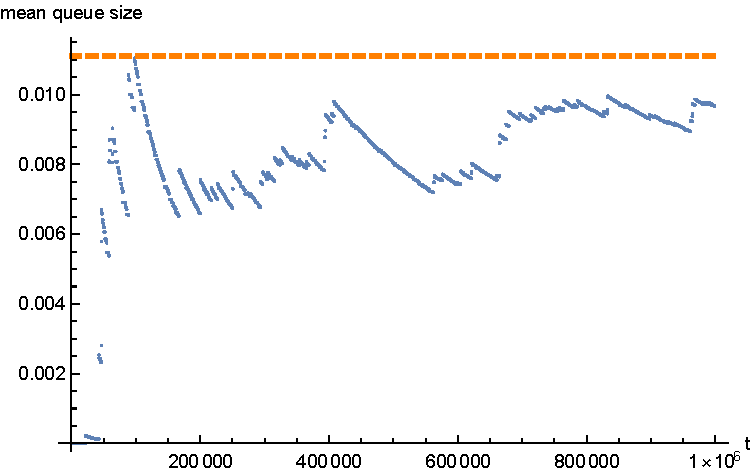
\includegraphics[width=0.8\textwidth]{abbildungen/1_Phone/Arrival_1000_Serve_100_dur_1000000_Skip_0/MeanQueueSize.pdf}
	\caption{Durchschnittliche Warteschlangenlänge, MeanAr = 1000}
	\label{fig:meanQueueSize1000}
\end{figure}

Bei der Betrachtung der in Abbildung \ref{fig:meanQueueSize1000} gezeigte durchschnittlichen Warteschlangenlänge fällt auf, dass die Werte zu Beginn der Simulation um ca. $0,004$ schwanken. Auch gegen Ende der Simulation schwanken die Werte noch um ca. $0,0018$. Während der gesamten Simulationsdauer liegen die Werte unter dem Erwartungswert von $0,0111111$, nähern sich diesem jedoch gegen Ende der Simulationszeit immer weiter an. Grund hierfür könnte ein nicht vollkommen eingeschwungenes System sein. Die Simulation müsste hierfür erneut durchgeführt werden, mit einer größeren Simulationsdauer.

\begin{figure}[htpb]
	\centering
	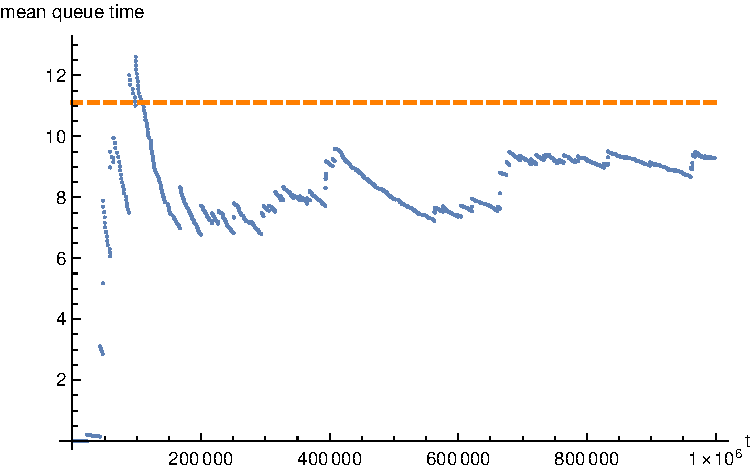
\includegraphics[width=0.8\textwidth]{abbildungen/1_Phone/Arrival_1000_Serve_100_dur_1000000_Skip_0/MeanQueueTime.pdf}
	\caption{Durchschnittliche Verweildauer in der Warteschlange , MeanAr = 1000}
	\label{fig:meanQueueTime1000}
\end{figure} 

Die in Abbildung \ref{fig:meanQueueTime1000} aufgeführte durchschnittliche Verweildauer in der Warteschlange weißt einen ähnlichen Verlauf auf wie die in Abbildung \ref{fig:meanQueueSize1000} gezeigte durchschnittliche Warteschlangenlänge. Dieses Verhalten ist plausibel, da bei einer größeren Warteschlangenlänge auch die Wartezeit in der Warteschlange steigt. Gegen Ende der Simulation näher sich die durchschnittliche Verweildauer in der Warteschlange dem Erwartungswert von $11,1111$ an, erreicht ihn jedoch nicht. Wie bereits erläutert müsste die Simulation für eine genauere Beurteilung erneut mit einer längeren Simulationsdauer durchgeführt werden. 

\begin{figure}[htpb]
	\centering
	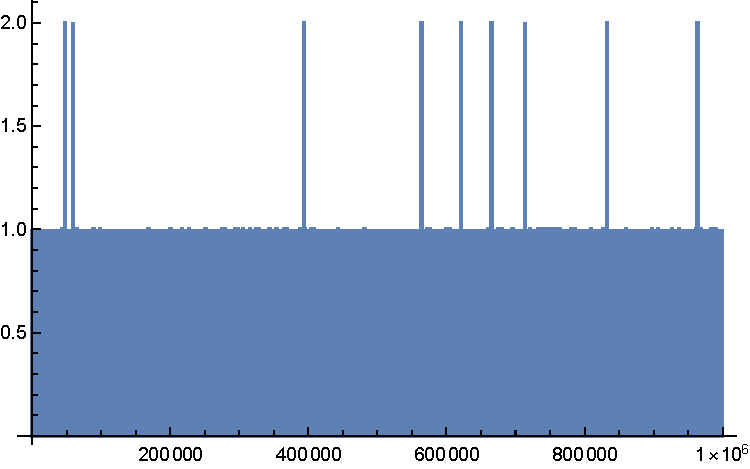
\includegraphics[width=0.8\textwidth]{abbildungen/1_Phone/Arrival_1000_Serve_100_dur_1000000_Skip_0/QueueStepPlotAll.pdf}
	\caption{Warteschlangenlänge (ungefiltert) , MeanAr = 1000}
	\label{fig:QueueStepPlotAll1000}
\end{figure} 
\begin{figure}[htpb]
	\centering
	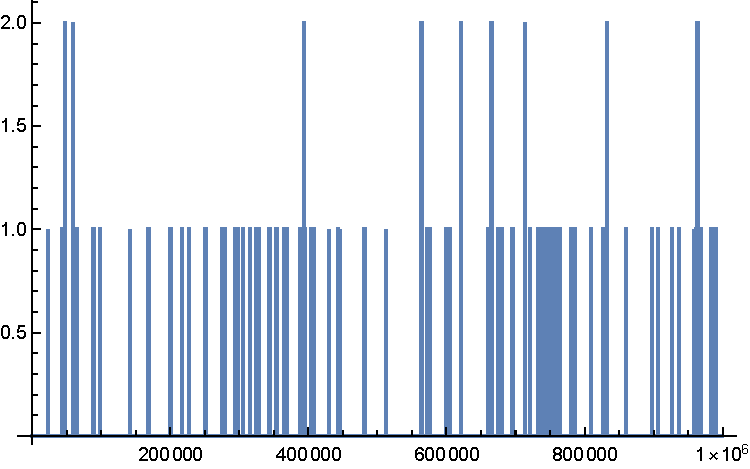
\includegraphics[width=0.8\textwidth]{abbildungen/1_Phone/Arrival_1000_Serve_100_dur_1000000_Skip_0/QueueStepPlotAllFiltered.pdf}
	\caption{Warteschlangenlänge (gefiltert) , MeanAr = 1000}
	\label{fig:QueueStepPlotAllFiltered1000}
\end{figure} 

Die Abbildung \ref{fig:QueueStepPlotAll1000} zeigt die einzelnen Werte für die Warteschlangenlänge über die Simulationszeit. Diese Abbildung ist nicht aussagekräftig. Hintergrund dafür ist die Implementierung der Simulation. Im Warteschlangenmodell wird zwischen drei verschiedenen Events unterschieden. Betritt ein neuer Kunde den Telefonshop, wird ein Arrival Event ausgelöst und die Warteschlangenlänge wird um 1 erhöht. Ist das Telefon frei, wird ein Begin Event ausgelöst und die Warteschlangenlänge wird um 1 reduziert. Hat ein Kunde sein Telefonat beendet, wird ein Finish Event ausgelöst, was wiederum ein Begin Event auslöst, da das Telefon frei ist. Ein Problem gibt es hierbei für den Fall, dass kein Kunde im Laden steht und somit auch die Warteschlange leer und das Telefon frei ist. Betritt nun ein neuer Kunde den Laden, wird ein Arrival Event ausgelöst und direkt anschließend ein Begin Event, da das Telefon frei ist und der Kunde sein Telefonat sofort beginnen kann. Er befindet sich somit für $0s$ in der Warteschlange. Aufgrund der Events wird die Warteschlangenlänge jedoch trotzdem erhöht und direkt wieder gesenkt. Es gibt somit für den gleichen Zeitstempel zwei unterschiedliche Warteschlangenlängen. Abbildung \ref{fig:QueueStepPlotAllFiltered} zeigt die gleiche Situation ohne die eben erläuterte Situation. Es wird hierbei nur eine Warteschlangenlänge angezeigt, wenn auch wirklich ein Kunde länger als $0s$ in der Warteschlange wartet. Da das System nur sehr gering ausgelastet ist, ist die geringe Warteschlangenlänge plausibel.\\
Abschließend sind im folgenden die berechneten Werte für die durchschnittliche Warteschlangenlänge, Wartezeit in der Warteschlange, Anzahl an Clients im System und Zeit im System aufgeführt:
%\[\begin{array}{cc}
 \text{mean queue size} & 0.00537307572764891636692565082375430880024384373 \\
 \text{mean queue time} & 8.19291 \\
 \text{mean system size} & 0.06921258430823697932263116253494454280311475015 \\
 \text{mean system time} & 105.458 \\
\end{array}\]


FEHLT !!!!!!!!!!!!!!!!!!!!!!!!!!!!!
\paragraph{Validierung der Simulation}
\begin{figure}[htpb]
	\centering
	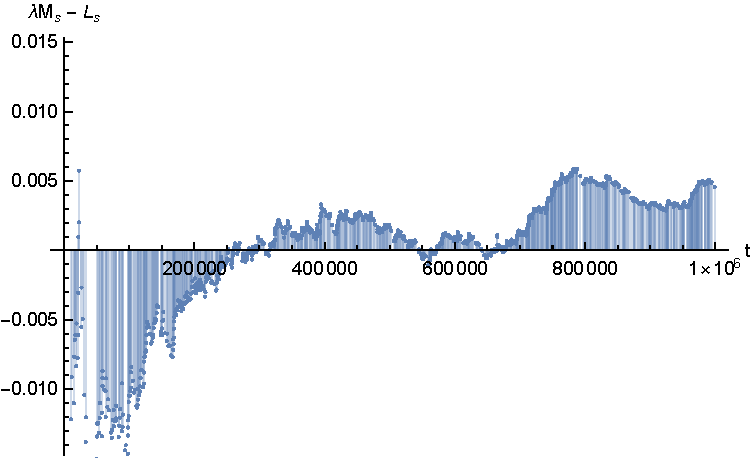
\includegraphics[width=0.8\textwidth]{abbildungen/1_Phone/Arrival_1000_Serve_100_dur_1000000_Skip_0/LittleSystem.pdf}
	\caption{Durchschnittliche Verweildauer in der Warteschlange , MeanAr = 1000}
	\label{fig:LittleSystem1000}
\end{figure} 
In Abbildung \ref{fig:LittleSystem1000} ist der Verlauf der Gleichung \ref{eq:little} über die Simulationszeit aufgeführt. Ab einer Simulationsdauer von ca. $350000$ liegt der Wert sehr nach an dem geforderten Erwartungswert von $0$, schwankt jedoch bis zum Ende der Simulation im Bereich von $0,004$. Darauf folgt, dass entweder ein Fehler in der Berechnung oder, was aufgrund der sehr geringen Abweichung vom Erwartungswert wahrscheinlicher ist, das System noch nicht vollständig eingeschwungen war. Für weitere Erkenntnisse müsste, wie bereits erwähnt die Simulation mit längerer Simulationsdauer erneut ausgeführt werden.  

%\subsubsection{Durchschnittliche Ankunftszeit der Clients: 500}
%\paragraph{Verwendung der Mathematica Simulation}
%- Bild der Simulation 
%- Plot Little-Law
%- MeanSystemSize, MeanSystemTime, MeanQueueSize,MeanQueueTime aufführen
%\paragraph{Verwendung der implementierten Java-Simulation, Berechnung in Mathematica}
%
%
%\paragraph{Simulation und Berechnung in Java}


\subsubsection{Durchschnittliche Ankunftszeit der Clients: 100}
\paragraph{Theoretische Erwartungswerte laut M/M/1 Warteschlangenmodell}
Für durchschnittliche Zwischenankunftszeit und durchschnittliche Telefonierdauer 100 ($\lambda=\frac{1}{100}$, $\mu=\frac{1}{100}$), lassen sich die durchschnittliche Warteschlangenlänge, Wartezeit in der Warteschlange, Anzahl an Clients im System und Zeit im System nicht berechnen. Die Warteschlangenlänge steigt gegen unendlich. Somit steigen auch die anderen drei Größen mit zunehmender Simulationsdauer gegen unendlich.

\paragraph{Verwendung der implementierten Java-Simulation, Berechnung in Java}
\begin{figure}[htpb]
	\centering
	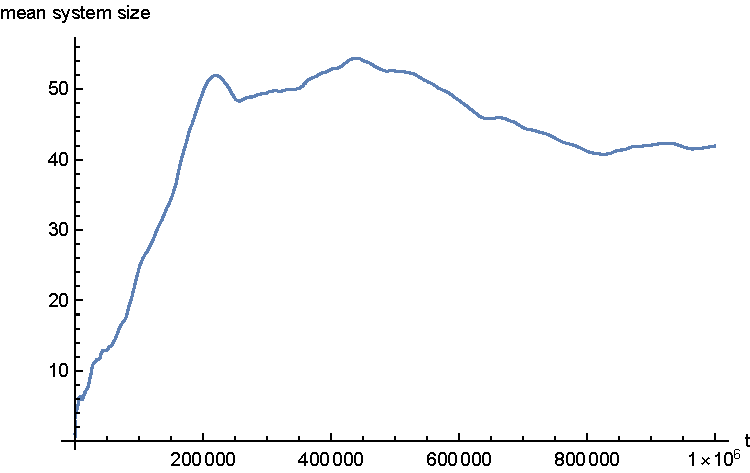
\includegraphics[width=0.8\textwidth]{abbildungen/1_Phone/Arrival_100_Serve_100_dur_1000000_Skip_0/MeanSystemSize.pdf}
	\caption{Durchschnittliche Anzahl an Kunden im System, MeanAr = 100}
	\label{fig:meanSystemSize100}
\end{figure}

\begin{figure}[htpb]
	\centering
	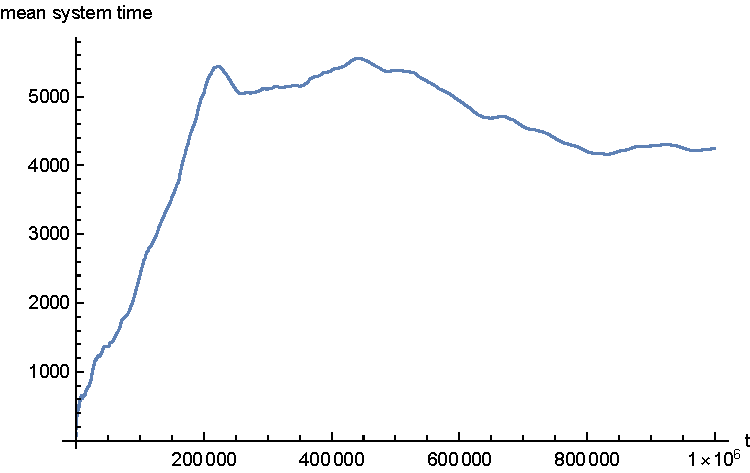
\includegraphics[width=0.8\textwidth]{abbildungen/1_Phone/Arrival_100_Serve_100_dur_1000000_Skip_0/MeanSystemTime.pdf}
	\caption{Durchschnittliche Verweildauer der Kunden im System, MeanAr = 100}
	\label{fig:meanSystemTime100}
\end{figure}

\begin{figure}[htpb]
	\centering
	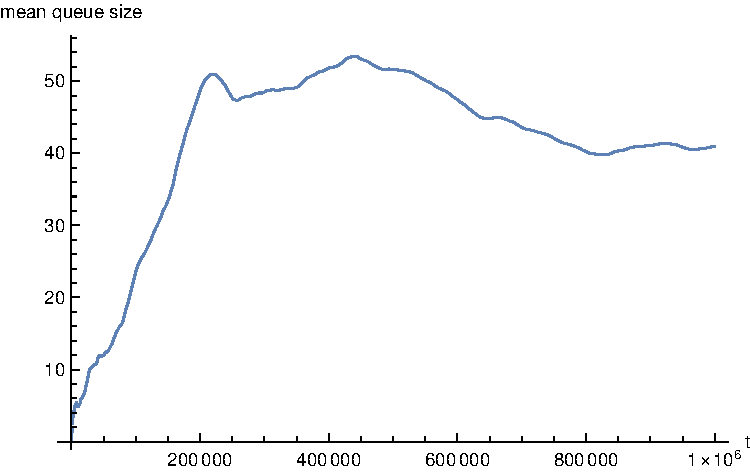
\includegraphics[width=0.8\textwidth]{abbildungen/1_Phone/Arrival_100_Serve_100_dur_1000000_Skip_0/MeanQueueSize.pdf}
	\caption{Durchschnittliche Warteschlangenlänge, MeanAr = 100}
	\label{fig:meanQueueSize100}
\end{figure}

\begin{figure}[htpb]
	\centering
	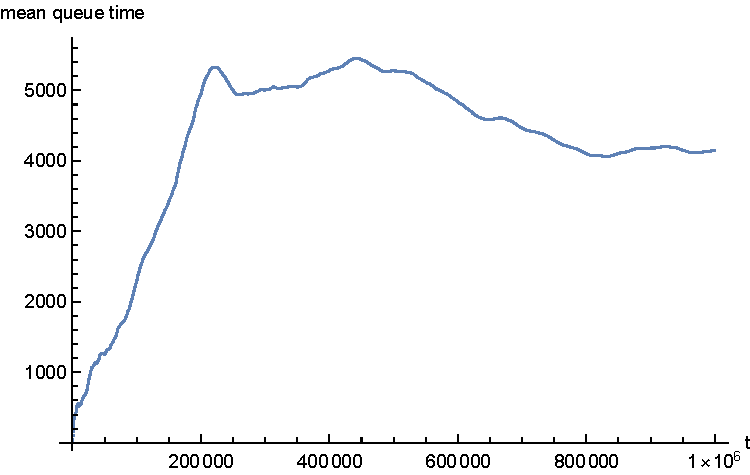
\includegraphics[width=0.8\textwidth]{abbildungen/1_Phone/Arrival_100_Serve_100_dur_1000000_Skip_0/MeanQueueTime.pdf}
	\caption{Durchschnittliche Verweildauer in der Warteschlange , MeanAr = 100}
	\label{fig:meanQueueTime100}
\end{figure} 

\begin{figure}[htpb]
	\centering
	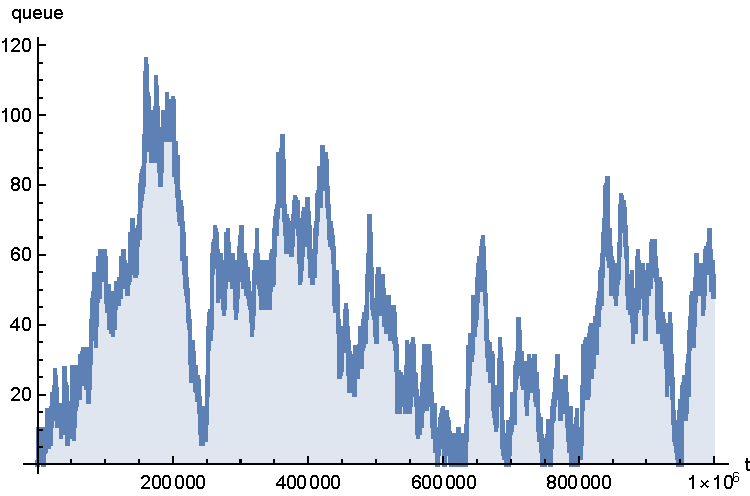
\includegraphics[width=0.8\textwidth]{abbildungen/1_Phone/Arrival_100_Serve_100_dur_1000000_Skip_0/QueueStepPlotAll.pdf}
	\caption{Warteschlangenlänge (ungefiltert) , MeanAr = 100}
	\label{fig:QueueStepPlotAll100}
\end{figure} 
\begin{figure}[htpb]
	\centering
	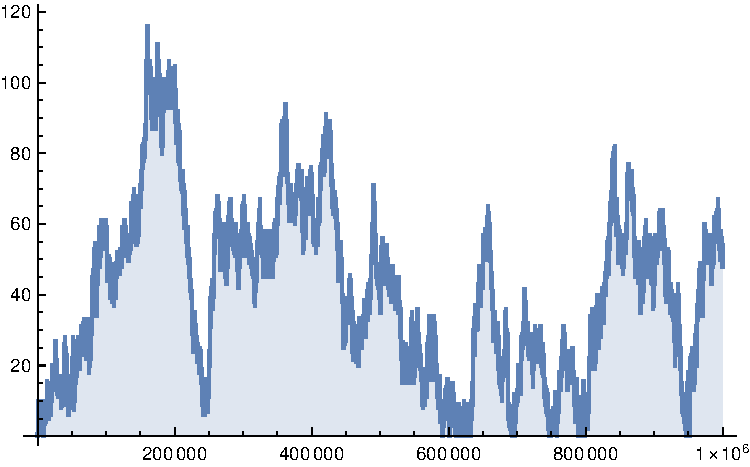
\includegraphics[width=0.8\textwidth]{abbildungen/1_Phone/Arrival_100_Serve_100_dur_1000000_Skip_0/QueueStepPlotAllFiltered.pdf}
	\caption{Warteschlangenlänge (gefiltert) , MeanAr = 100}
	\label{fig:QueueStepPlotAllFiltered100}
\end{figure} 
Abschließend sind im folgenden die berechneten Werte für die durchschnittliche Warteschlangenlänge, Wartezeit in der Warteschlange, Anzahl an Clients im System und Zeit im System aufgeführt:
%\[\begin{array}{cc}
 \text{mean queue size} & 0.00537307572764891636692565082375430880024384373 \\
 \text{mean queue time} & 8.19291 \\
 \text{mean system size} & 0.06921258430823697932263116253494454280311475015 \\
 \text{mean system time} & 105.458 \\
\end{array}\]


FEHLT !!!!!!!!!!!!!!!!!!!!!!!!!!!!!

\paragraph{Validierung der Simulation}
\begin{figure}[htpb]
	\centering
	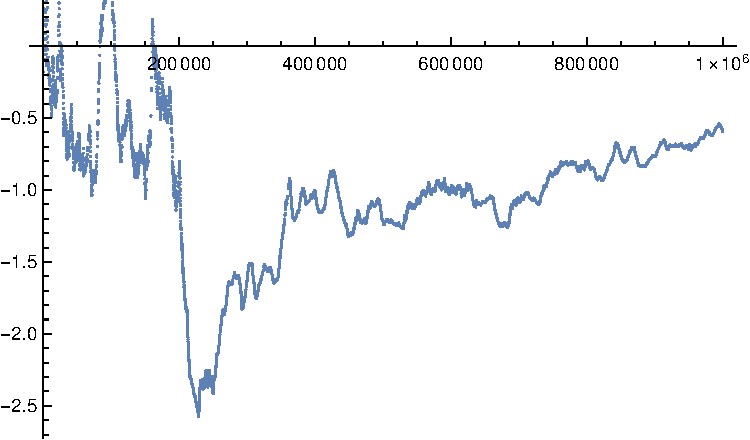
\includegraphics[width=0.8\textwidth]{abbildungen/1_Phone/Arrival_100_Serve_100_dur_1000000_Skip_0/LittleSystem.pdf}
	\caption{Durchschnittliche Verweildauer in der Warteschlange , MeanAr = 1000}
	\label{fig:LittleSystem100}
\end{figure} 
In Abbildung \ref{fig:LittleSystem1000} ist der Verlauf der Gleichung \ref{eq:little} über die Simulationszeit aufgeführt.
\subsection{Modell \glqq Bevorzugte VIP\grqq} 
\subsubsection{Durchschnittliche Ankunftszeit der Clients: 100}
\subsubsection{Durchschnittliche Ankunftszeit der Clients: 500}
\subsubsection{Durchschnittliche Ankunftszeit der Clients: 1000}
\subsubsection{Durchschnittliche Ankunftszeit der Clients: 1500}

\subsection{Modell \glqq Zusätzliches VIP Telefon\grqq} 
\subsubsection{Durchschnittliche Ankunftszeit der Clients: 100}
\subsubsection{Durchschnittliche Ankunftszeit der Clients: 500}
\subsubsection{Durchschnittliche Ankunftszeit der Clients: 1000}
\subsubsection{Durchschnittliche Ankunftszeit der Clients: 1500}

\section{Fazit}

\end{document}
